\documentclass{standalone}
\usepackage{tikz}
\usepackage{pgfplots}

\tikzset{align at bottom/.style={baseline=(current bounding box.south)}}

\begin{document}
	\begin{tikzpicture}[scale = 0.27]
	
		\begin{scope}
			\clip (-5, -5) rectangle (5, 5);
%			\clip (-4.5, -4.5) rectangle (4.5, 4.5);
			\node[anchor = center, inner sep = 0, opacity = 1] at (0, 0) {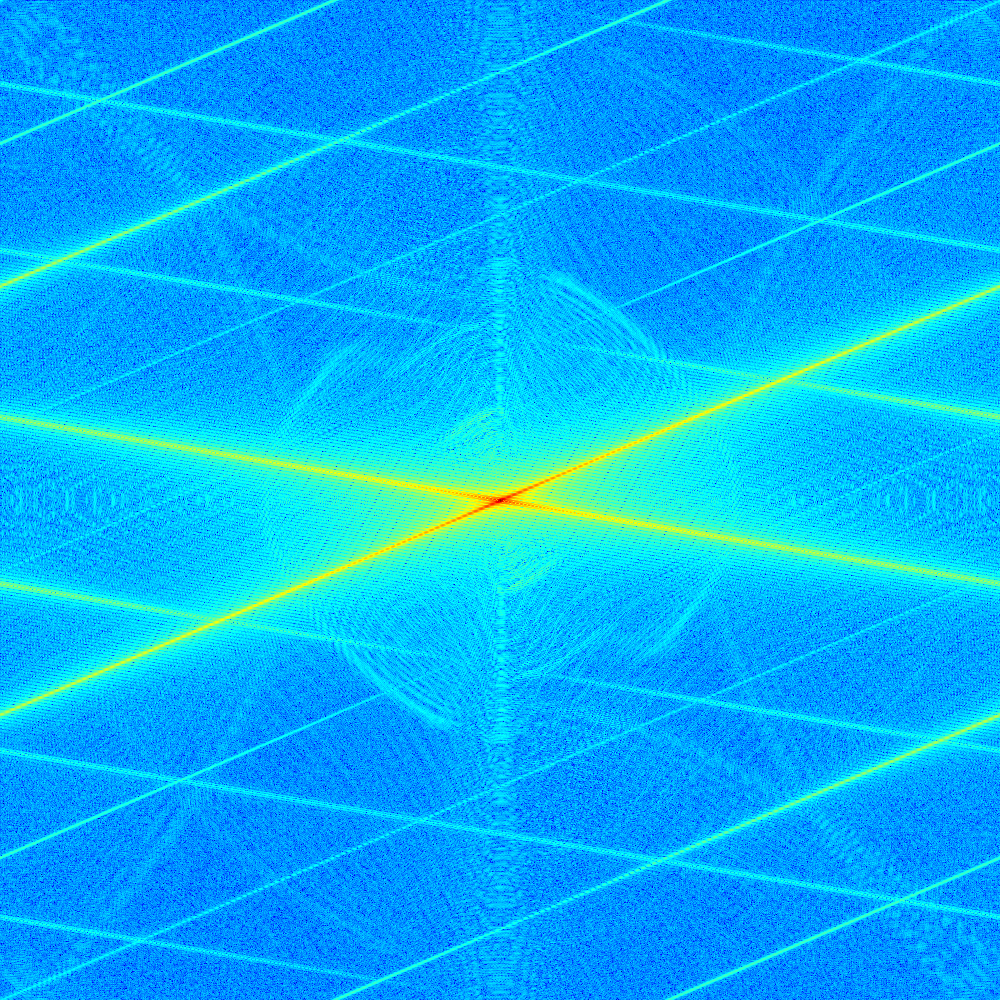
\includegraphics[width = 5cm]{figures/spectral_support/fft_red_and_blue.png}};
		\end{scope}
		
		\begin{scope}
			\draw[->, opacity = 1] (-5, 0) -- (5, 0) node[right, opacity = 1] {$\xi_s$};
			\draw[->, opacity = 1] (0, -5) -- (0, 5) node[above, opacity = 1] {$\xi_u$};
		\end{scope}
		
		% Invisible dummy node for symmetric alignment with caption
		\node[left, opacity = 0] at (-5, 0) {$\xi_s$};
		
	\end{tikzpicture}
\end{document}